\documentclass{article}

% if you need to pass options to natbib, use, e.g.:
% \PassOptionsToPackage{numbers, compress}{natbib}
% before loading nips_2018

% ready for submission
\usepackage[preprint]{nips_2018}
\usepackage{graphicx}

% to compile a preprint version, e.g., for submission to arXiv, add
% add the [preprint] option:
% \usepackage[preprint]{nips_2018}

% to compile a camera-ready version, add the [final] option, e.g.:
% \usepackage[final]{nips_2018}

% to avoid loading the natbib package, add option nonatbib:
% \usepackage[nonatbib]{nips_2018}

\usepackage[utf8]{inputenc} % allow utf-8 input
\usepackage[T1]{fontenc}    % use 8-bit T1 fonts
\usepackage{hyperref}       % hyperlinks
\usepackage{url}            % simple URL typesetting
\usepackage{booktabs}       % professional-quality tables
\usepackage{amsfonts}       % blackboard math symbols
\usepackage{nicefrac}       % compact symbols for 1/2, etc.
\usepackage{microtype}      % microtypography

\title{[EE240] Preliminary project report\\Simple Smart-Driving Skill Evaluation System}

% The \author macro works with any number of authors. There are two
% commands used to separate the names and addresses of multiple
% authors: \And and \AND.
%
% Using \And between authors leaves it to LaTeX to determine where to
% break the lines. Using \AND forces a line break at that point. So,
% if LaTeX puts 3 of 4 authors names on the first line, and the last
% on the second line, try using \AND instead of \And before the third
% author name.

\author{
  Yuan-Pu Hsu \\\#862057597\\
  \And 
  Tianxiang Sun\\\#862051319\\
  %% \texttt{hippo@cs.cranberry-lemon.edu} \\
  %% examples of more authors
  %% \And
  %% Coauthor \\
  %% Affiliation \\
  %% Address \\
  %% \texttt{email} \\
  %% \AND
  %% Coauthor \\
  %% Affiliation \\
  %% Address \\
  %% \texttt{email} \\
  %% \And
  %% Coauthor \\
  %% Affiliation \\
  %% Address \\
  %% \texttt{email} \\
  %% \And
  %% Coauthor \\
  %% Affiliation \\
  %% Address \\
  %% \texttt{email} \\
}

\begin{document}
% \nipsfinalcopy is no longer used

\maketitle

% \begin{abstract}

% \end{abstract}

\section{Introduction}

Nowadays, over 90\% of families in America own at least one vehicle. Driving has already been a big portion of American’s daily life for decades. Therefore, we want to make a simple system to evaluate the driving skill of the driver. The user will get a score of their driving skill after finishing a tour, and the only thing needed is a smart phone. We believe it can help drivers to evaluate their driving skill and improve their skill to some extent. Furthermore, insurance company can also use the score to evaluate the credit of their clients, while those who has better driving skill should be benefited with lower insurance bill.

When it comes to the details, we want to build an app in the smart phone (in our case, iPhone). The user can place the device behind the front windscreen, and let it automatically analyze the image and recognize different patterns on the road. In this project, we restrict the targets within the vision to traffic lights, stop signs, speed limit signs, and pedestrians. Besides, we will take advantage of the GPS and accelerometer on the phone to calculate the speed and acceleration of the car. After comparing the speed of the car and patterns gotten by the mobile device, we can evaluate his/her driving score by the information. For example, if the user did not slow down while meeting a pedestrian, he/she would lose some points; if the user drive smoothly for a period of time, he/she would gain some points.

There are several researches regarding to recognition of traffic signs as listed in the reference. Mainly, we are going to implement Convolutional Neural Network (CNN) for pattern recognition with the method by Shustanov, A. et al. [4], Habibi Aghdam, H,. et al. [2], and optimize the speed for real-time scenario with the method of Kardkovacs, Z. et al. [3] We want to use the dataset called German Traffic sign benchmark as the training set of traffic signs. On the other hand, we are using cascade classifier by Angelova, A. et al. [1] to detect pedestrians for low latency with Caltech dataset. We will utilize the common tools for implementing computer vision and machine learning like TensorFlow, and AWS to build the proposed system. Meantime, we would also compare the efficiency of computation under different real-time scenario, such as whether compute locally with GPU on the phone, or upload to the cloud via LTE.

\section{Implementation}
The implementation of our project can be separate to three parts: iOS application (deploy on iPhone6s), Amazon Web Services (AWS) with TensorFlow for speed-up development and accessing GPU computation, and the core CNN model for recognition. The system flow chart is shown in Figure 1.
% \begin{figure}[h]
%   \centering
%   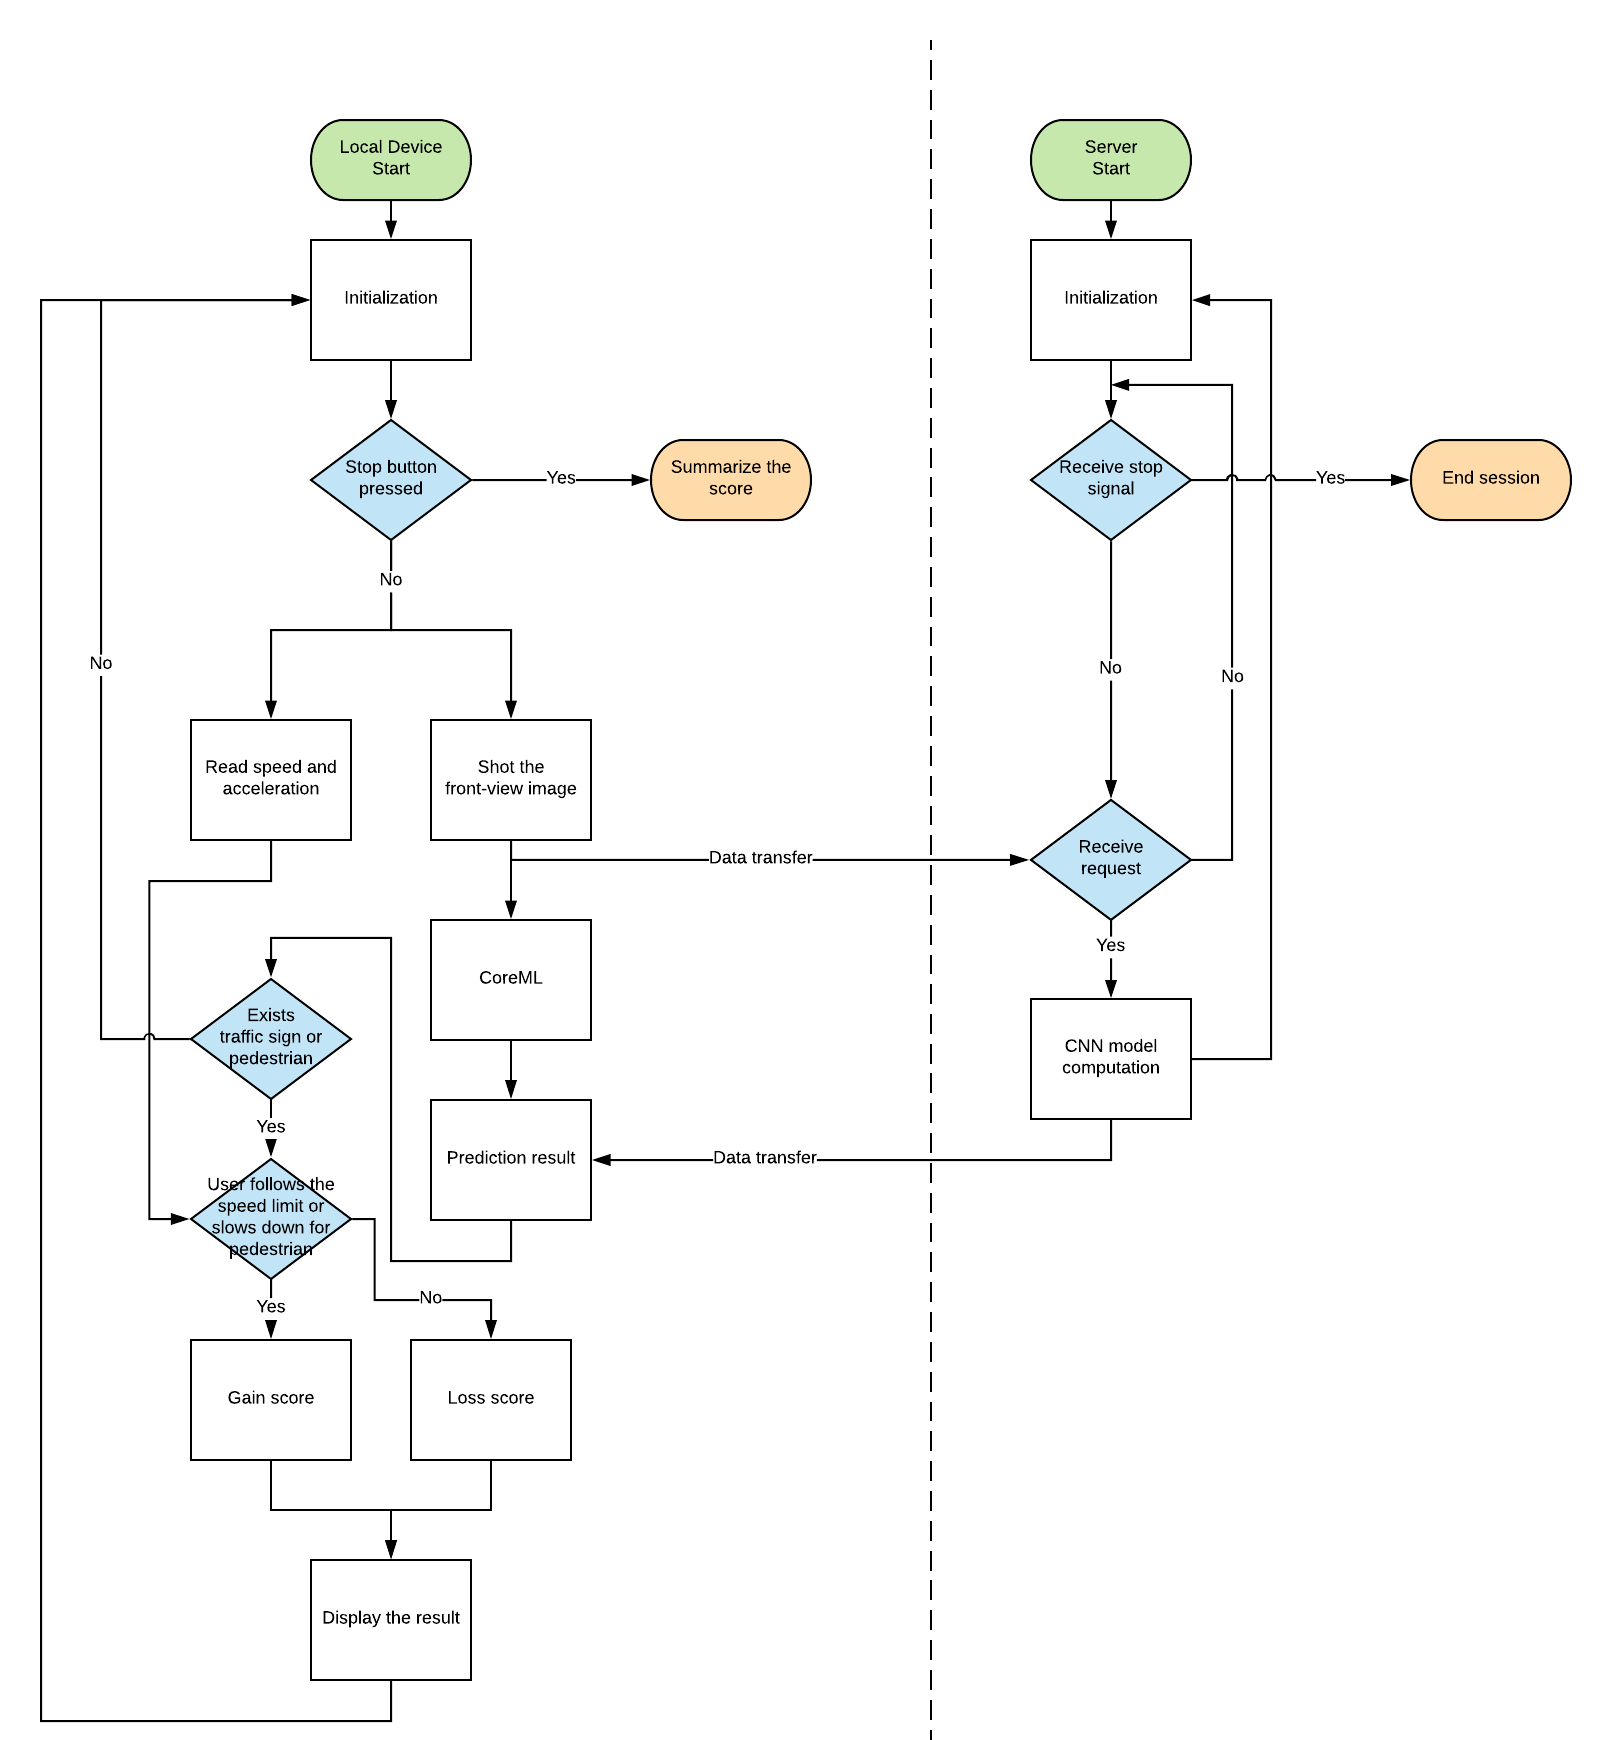
\includegraphics[width=\linewidth]{system_flowchart.png}
%   \caption{System flowchart}
% \end{figure}
\begin{figure}[ht]
  \centering
  \begin{minipage}{.4\textwidth}
    \centering
    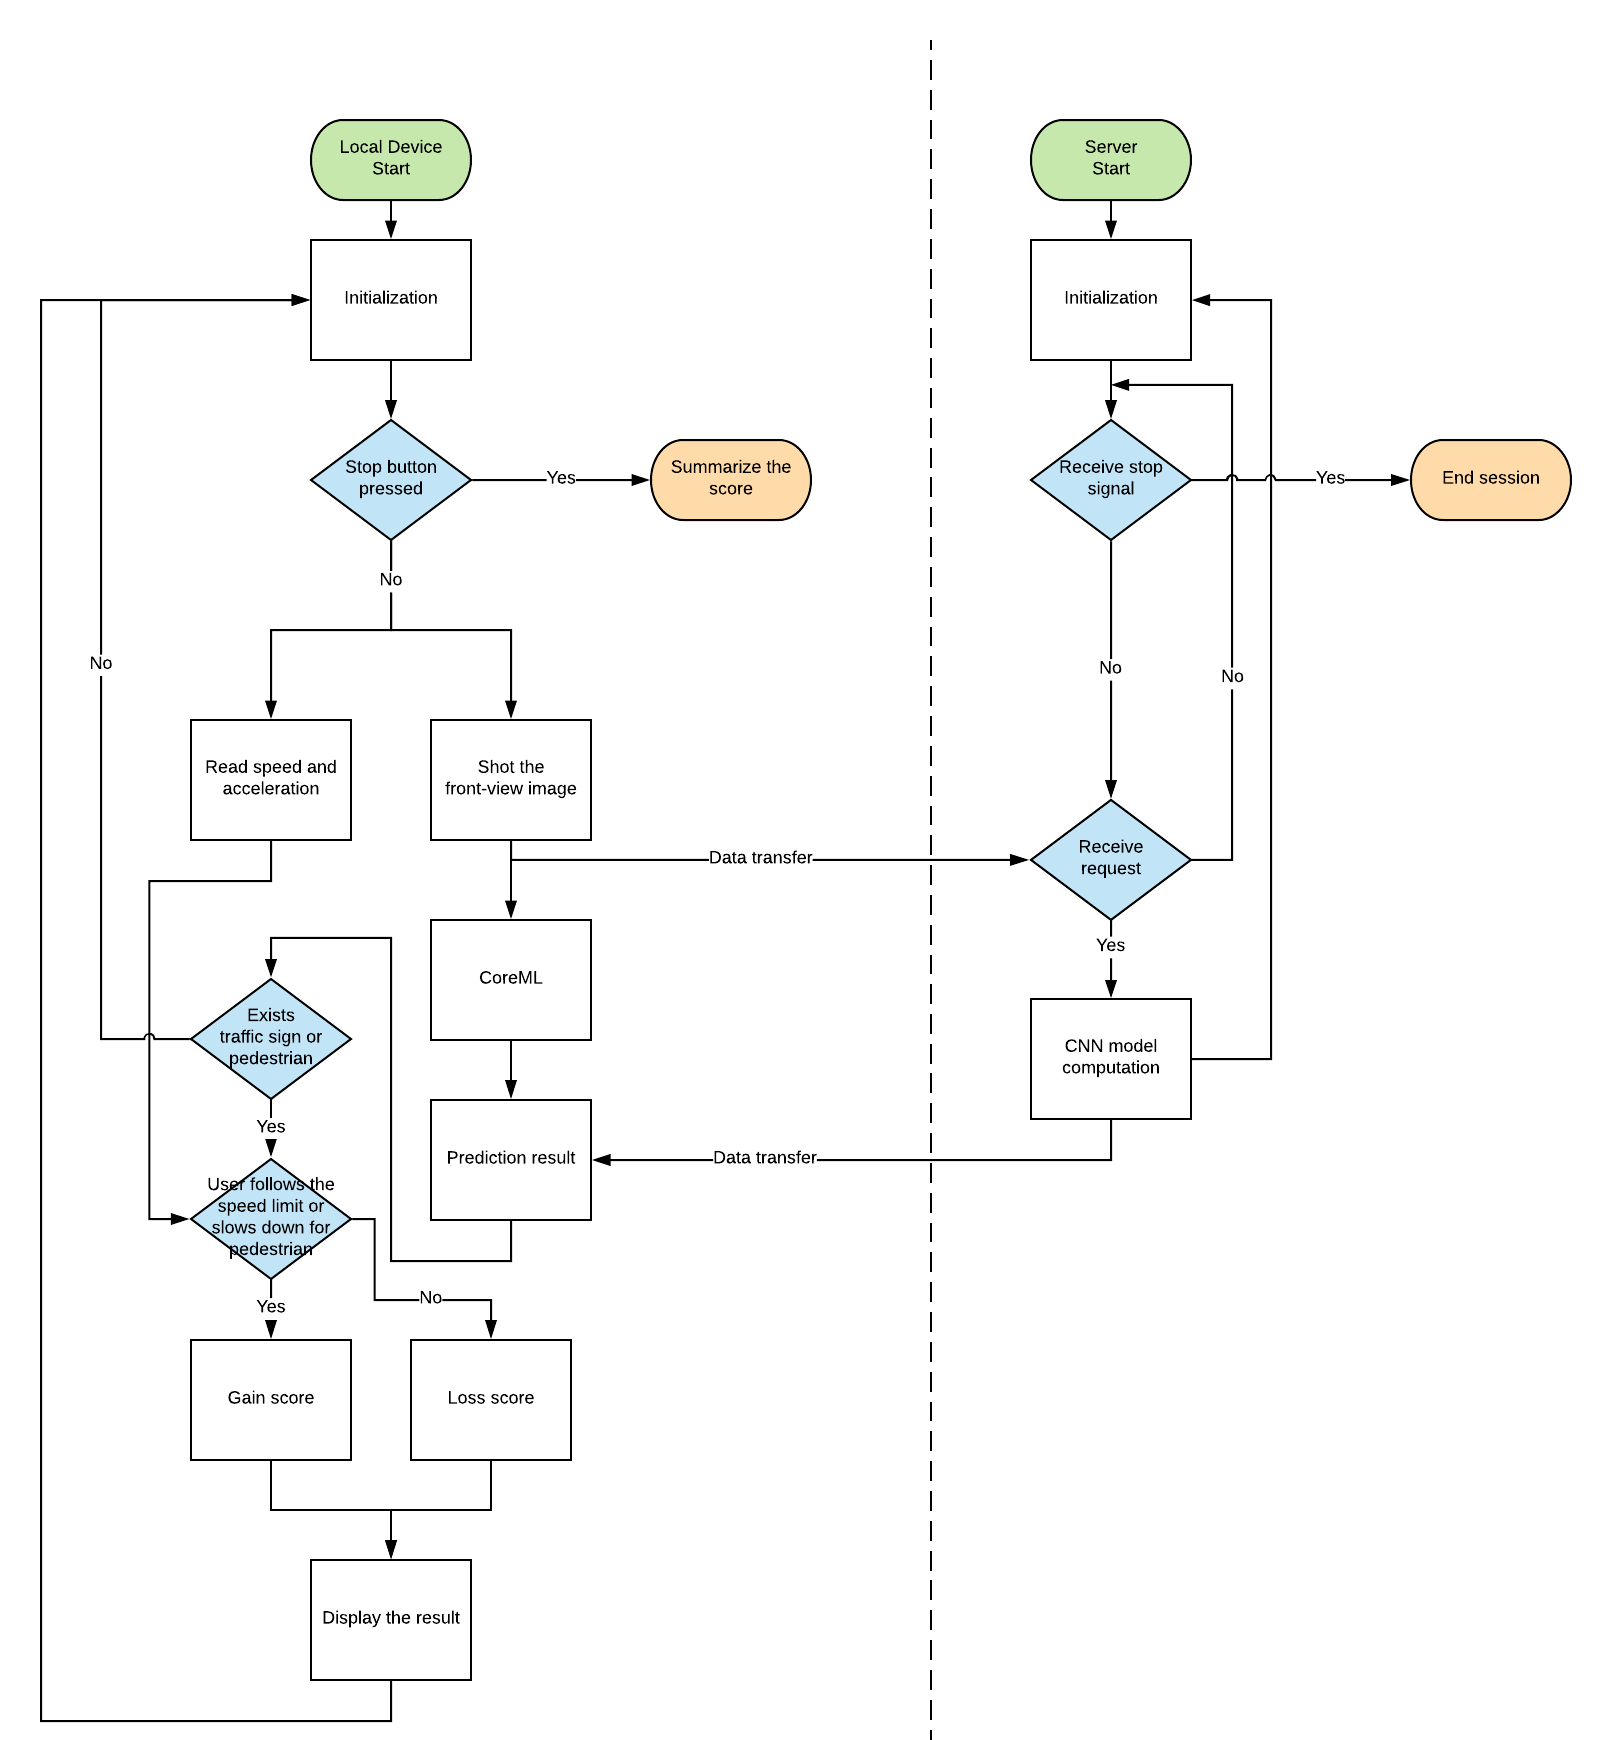
\includegraphics[width=1.2\linewidth]{system_flowchart.png}
    \caption{System design flowchart}
    \label{fig:fig_1}
  \end{minipage}
  \begin{minipage}{.4\textwidth}
    \centering
    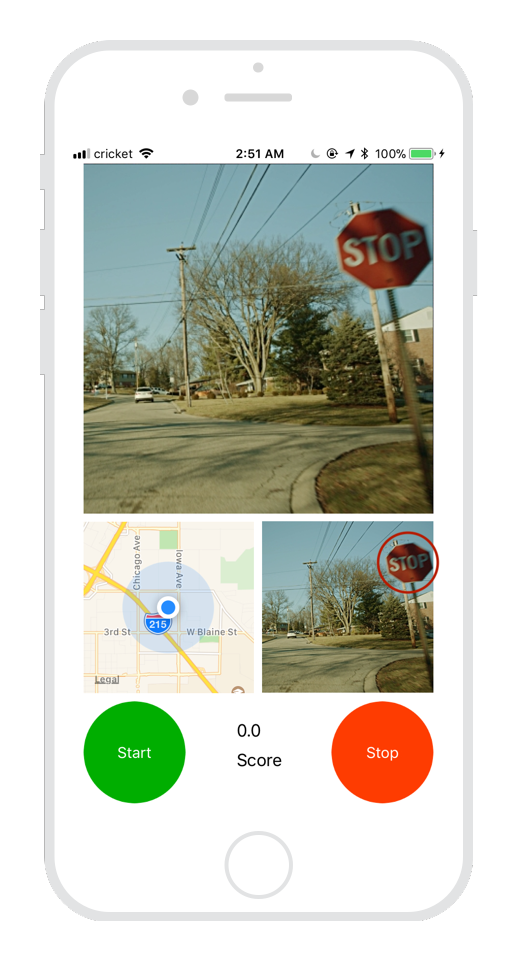
\includegraphics[width=.6\linewidth]{iOS_design.png}
    \caption{iOS app design}
    \label{fig:fig_2}
  \end{minipage}
\end{figure}
\subsection{iOS Application}
We first build a simple app for taking the front-view picture periodically, and record both the speed and acceleration at the same time via MapKit. The picture will then pass through the trained CNN model installed in the bundle, or upload to the cloud service for the prediction. The result includes whether there existed a traffic sign or pedestrian in the picture, and what kind of sign it is. After the translation of the speed limit is done, the app can determine if the user was over speed. In the end, the app would give the user a high score if he/she follows the signs and slow down for the pedestrian and vise versa.

\subsection{AWS Server with TensorFlow}
We build a Ubuntu virtual machine on the AWS server with both CPU and GPU deployment. In the machine, we installed tools like Python, TensorFlow and CUDA, etc., for fast implementation of train and tune the CNN model. After the model was trained on the server, we On the other hand, the server would allow the local device to upload the input image for prediction and then pass back the result of prediction after the computation.

\subsection{Convolution Neural Network Model}
\subsubsection{Preprocessing}
Here we are using German Traffic Sign Benchmark (GTSB) as the training set, which contains 43 kinds of different traffic signs with around 34000 images in the set. The training set would first be processed with mean, centering, normalizing, and histogram equalizing to help accelerating the train process in the later section. In addition, for augmenting the dataset, we also applied rotating and mirroring to mimic more possibilities in the real world cases. Then separate into 3 sets: training set, validating set and testing set in order to train the model. The distribution of each class of data is shown in Figure 3, and three kinds of the common type of sign images in the dataset is shown in Figure 4.

\begin{figure}[ht]
  \centering
  \begin{minipage}{.5\textwidth}
    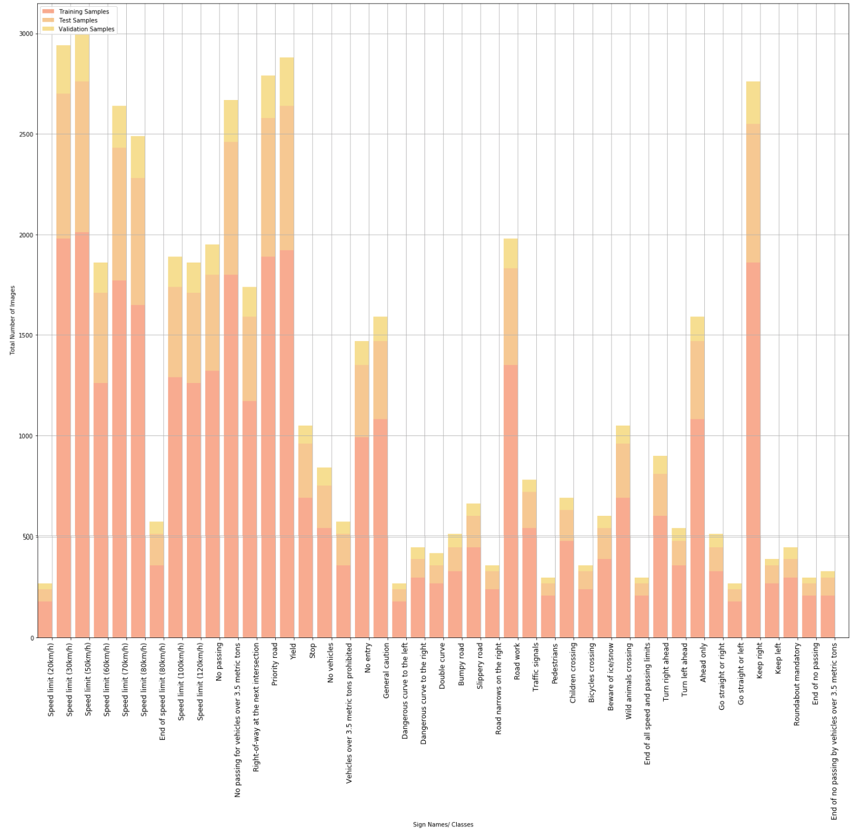
\includegraphics[width=1\linewidth]{data_distribution.png}
    \caption{Data distribution}
    \label{fig:fig_3}
  \end{minipage}
  \begin{minipage}{.4\textwidth}
    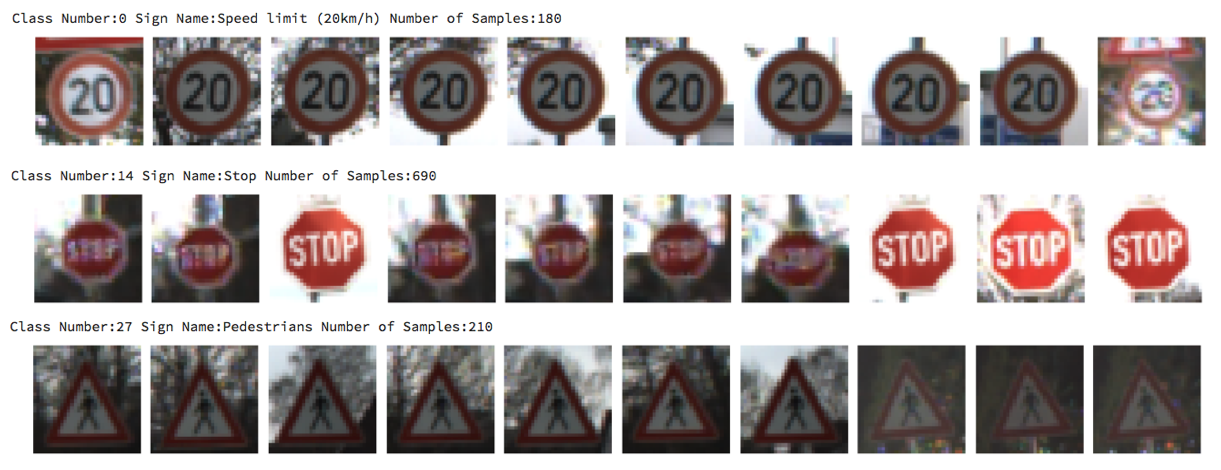
\includegraphics[width=1.5\linewidth]{signs_data.png}
    \centering
    \caption{Images of the traffic signs}
    \label{fig:fig_4}
  \end{minipage}
\end{figure}

\subsubsection{Model Architecture}
We would construct our own CNN model based on VGG Net [5], with a linear classifier. Specifically, we adopted VGG-5 architecture with four VGG convolution layers, a multi scale concatenate layer, two fully connected  layers and a logits layer. With the multi scale architecture that subsampling the output of each VGG block and concatenate before fully connected layer, the lower order feature in the image would still be possible to vote for the final result. While the traffic-sign feature in our scenario might serve as a small part in the whole image, this way should be a better approach to treat those and have more accurate results. Besides, we also implement Spatial Transformers for achieve invariance in scale, and the Softmax activation function for classification. 

\subsubsection{Model Training}
In order to train the CNN model more efficiently, we use the AWS EC2 server to conduct all the complex computation. We would tune the learning rate, number of iterations, batch size, number of epochs, dropout rate, and regularization factor, etc., to construct a reliable model structure.

\section{Proceeding works}
After completing the training process, we would conduct the model into experiment. Our model would be translate into coreML model for implementation on the iOS device. To test computation speed and accuracy both on the cloud service and local device. On the other hand, we would also work on speed-up and optimize the model for securing real-time scenario.
% \subsubsection{Model Testing}


\section*{References}

% References follow the acknowledgments. Use unnumbered first-level
% heading for the references. Any choice of citation style is acceptable
% as long as you are consistent. It is permissible to reduce the font
% size to \verb+small+ (9 point) when listing the references. {\bf
%   Remember that you can use more than eight pages as long as the
%   additional pages contain \emph{only} cited references.}
\medskip

\small

[1] Angelova,A., Krizhevsky, A., Vanhoucke, V. Real-Time Pedestrian Detection With Deep Network Cascades. {\it Google research.}

[2] Habibi Aghdam,H., Jahani Heravi,E., Puig,D. (2016) A practical Approach for Detection and Classification of Traffic signs using Convolutional Neural Networks. {\it Robotics and Autonomous System}, Vol. 84, pp. 97-112.

[3] Kardkovacs, Z.T., Paroczi, Z.,Siegler,A.,(2011) Real-Time Traffic Sign Recognition System. {\it 2nd International Conference on Cognitive Infocommunications.}

[4] Shustanov, A., Yakimov, P., (2017). CNN Design For Real-Time Traffic Sign Recognition. {\it Procedia Engineering.} Vol.201,pp.718-725.

[5] Simonyan, K., Zisserman, A., (2014). Very Deep Convolutional Networks for Large-Scale Image Recognition. {\it ARXIV.} eprint arXiv:1409.1556

%% Zhu, Y.Y., Zhang, C.Q., Zhou, D.Y., Wang, X.G., Bai, X., Liu, W.Y., (2016) Traffic Sign Detection and Recognition Using Fully Convolutional Network Guided Proposals. {\it Neurocomputing.} Vol.214,pp.758-766.

%% Hasselmo, M.E., Schnell, E.\ \& Barkai, E.\ (1995) Dynamics of
%% learning and recall at excitatory recurrent synapses and cholinergic
%% modulation in rat hippocampal region CA3. {\it Journal of
%% Neuroscience} {\bf 15}(7):5249-5262.

\end{document}